\documentclass[12pt, letterpaper, fleqn]{article}
\usepackage[letterpaper, margin=.75in]{geometry}
\usepackage[utf8]{inputenc}
\usepackage{amsmath}
\usepackage{amssymb}
\usepackage{algorithmicx}
\usepackage{algpseudocode}
\usepackage{algorithm}
\usepackage[english]{babel}
\usepackage{amsthm}
\usepackage{graphicx}
\usepackage{xcolor}
\graphicspath{ {.} }
\usepackage{fancyhdr}
\usepackage{tikz}
\usepackage{hyperref}
\newcommand*\circled[1]{\tikz[baseline=(char.base)]{
            \node[shape=circle,draw,inner sep=2pt] (char) {#1};}}
\setlength\parindent{0pt}

%\pagestyle{fancy}
%\fancyhf{}
%\rhead{Bill Yang}
%\renewcommand{\headrulewidth}{0pt}

\newcommand{\handout}[5]{
   \renewcommand{\thepage}{#1-\arabic{page}}
   \noindent
   \begin{center}
   \framebox{
      \vbox{
%    \hbox to 5.78in { {\bf M328K Number Theory} \hfill #2 }
%       \vspace{4mm}
%       \hbox to 5.78in { {\Large \hfill #5  \hfill} }
%       \vspace{2mm}
%       \hbox to 5.78in { {\it #3 \hfill #4} }
    \hbox to 5.78in { { Bill Yang} \hfill {Due: #2} }
       \vspace{4mm}
       \hbox to 5.78in { {\Large \hfill #5  \hfill} }
       \vspace{2mm}
       \hbox to 5.78in { {#3 \hfill #4} }
      }
   }
   \end{center}
   \vspace*{4mm}
}

\newcommand{\ho}[5]{\handout{#1}{#2}{#3}{Instructor: #4}{Homework #1}}

\begin{document}
  \ho{6a}{3/13/19}{CS386D Database Systems}{Daniel Miranker} \\
  
  \textbf{1}\\
  a) \\\\
  In Seconds\\
  \begin{center}
  \begin{tabular}{ |c|c|c|c|c|c|c|c|c| }
   \hline
         & \multicolumn{2}{|c|}{Load Time} & \multicolumn{2}{|c|}{Query 1} &
         \multicolumn{2}{|c|}{Query 2} & \multicolumn{2}{|c|}{Query 3} \\
   \hline
   Data Generator & I & II & I & II & I & II & I & II \\
   \hline
   physical organization &      &     &      &     &     &     &    &  
   \\
   \hline
   1 & 746.5 & 799.9 & .2823 & .3901 & .2533 & .3319 & .1858 & .3156\\
   \hline
   2 & 870.9 & 1216.6 & .0215 & .0192 & .2185 & 6.4575 & .0136 & .017\\
   \hline
   3 & 886.2 & 971.2 & .225  & 3.1577 & .0199 & .0242 & .0119 & .0138\\
   \hline
   4 & 1017.8 & 1593.1 & .0279 & .0213 & .0211 & .0289 & .0137 & .0146 \\
   \hline
  \end{tabular}
  \end{center}


  b) \\
  \begin{center}
  \begin{tabular}{ |c|c|c|c|c|c|c|c|c| }
   \hline
         & \multicolumn{2}{|c|}{Load Time} & \multicolumn{2}{|c|}{Query 1} &
         \multicolumn{2}{|c|}{Query 2} & \multicolumn{2}{|c|}{Query 3} \\
   \hline
   Data Generator & I & II & I & II & I & II & I & II \\
   \hline
   physical organization &      &     &      &     &     &     &    &  
   \\
   \hline
   1 & 1     & 1.072 & 1    & 1.382 & 1     & 1.310  & 1     & 1.699\\
   \hline
   2 & 1.167 & 1.630 & .076 & .068  & .863  & 25.493 & .073  & .091\\
   \hline
   3 & 1.187 & 1.301 & .797 & 11.186& .079  & .096   & .064  & .074\\
   \hline
   4 & 1.363 & 2.134 & .099 & .075  & .083  & .114   & .074  & .079 \\
   \hline
  \end{tabular}
  \end{center}

  \textbf{2}\\
  For loading, a sequential load outperforms random insertion by a significant
  factor; even the queries benefit from the sequential load as well. Adding more
  indexes increases the insertion time for any data generator. Having an index
  greatly increases the speed in which queries execute if the condition of the
  query contains the attribute with an index. If there is no index for that
  attribute, but there exists another index on a different attribute, this may
  actually slow down the overall query eg. (Query 1, Data Generator 2, physical
  organization 3) and (Query 2, Data Generator 2, physical organization 2).
  These two setups and queries have a condition on attribute A and B, Random
  Generator, and indexes on B and A respectively.
  
  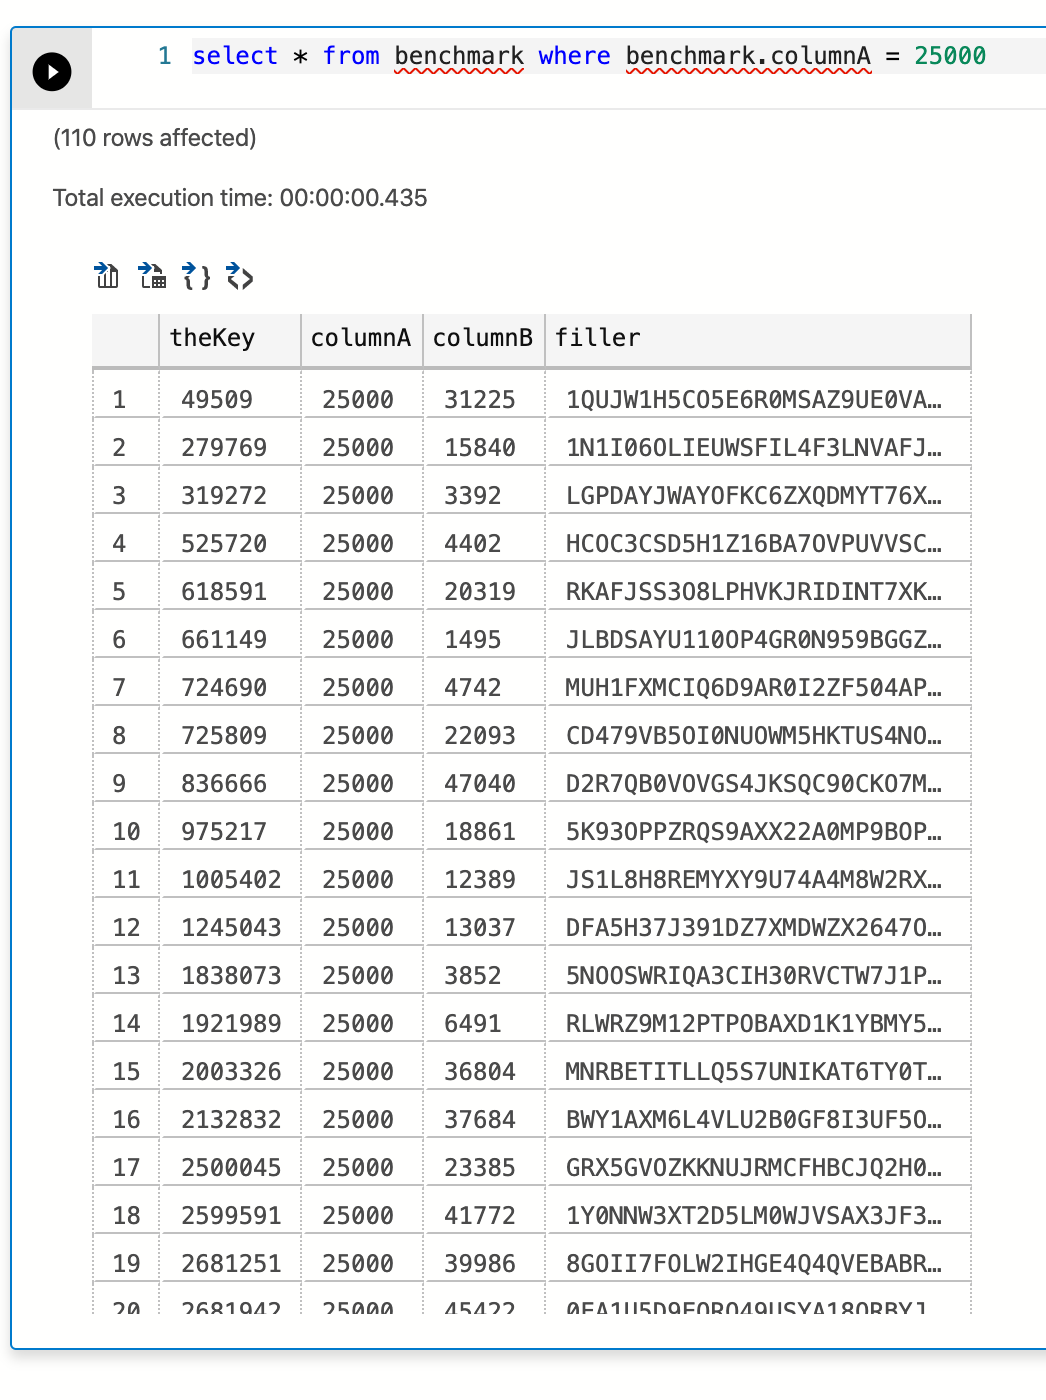
\includegraphics[scale=0.5]{queryAex}

 


\end{document}
